\section{Regulator DMC}

-------POLECENIE--------

Napisac program w jezyku MATLAB do symulacji algorytm DMC w najprostszej
wersji analitycznej. Dobrac parametry D, Nu, N i lambda algorytmu DMC przy skokowej
zmianie sygnału wartosci zadanej z 0 do 1 i zerowym zakłóceniu. Jakosc regulacji
oceniac jakosciowo (na podstawie rysunków przebiegów sygnałów) oraz ilosciowo, wyznaczajac
wskaznik jakosci regulacji
E =
kXkonc
k=1
$(yzad(k) - y(k))2$
gdzie kkonc oznacza koniec symulacji (zawsze taki sam). Zamiescic wybrane wyniki
symulacji (przebiegi sygnałów wejsciowych i wyjsciowych procesu oraz wartosci wskaznika
E).

to samo co w proj 1

-------POLECENIE--------


Algorytm DMC (Dynamic Matrix Control) algorytm regulacji predykcyjnej. 
Do predykcji wykorzystuje się model procesu w postaci odpowiedzi skokowych. 
W algorytmie DMC dynamika obiektu regulacji modelowana jest dyskretnymi odpowiedziami skokowymi, 
które opisują reakcję wyjścia na skok jednostkowy sygnału sterującego.
 
% \begin{figure}[H]
%     \centering
%     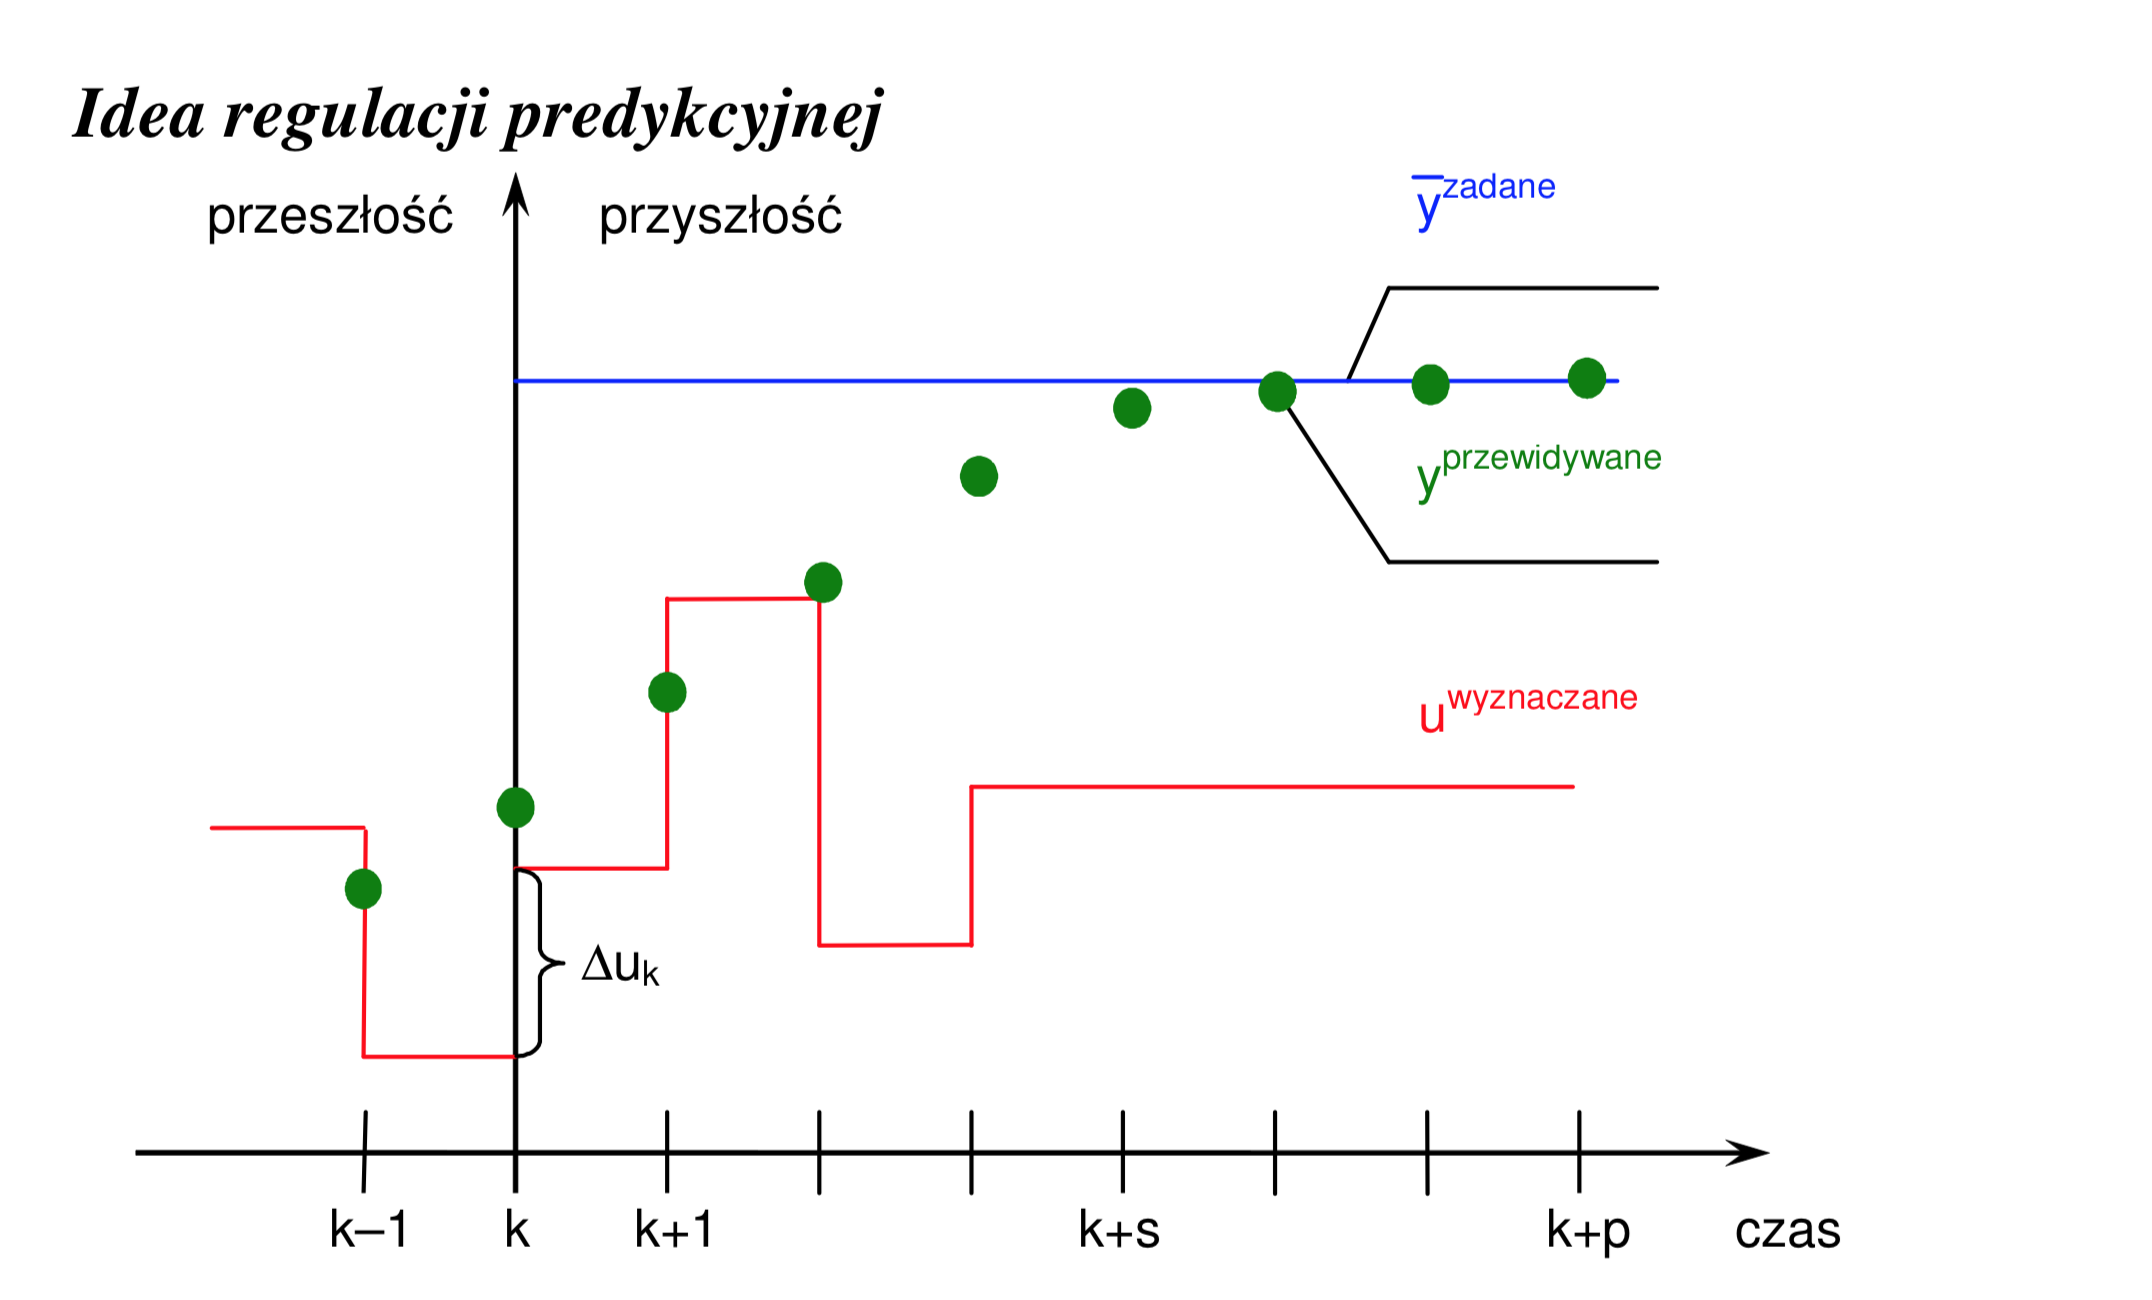
\includegraphics[scale=0.25]{dmc_idea.png}
%     \caption{Idea działania regulatora DMC}
% \end{figure}


\subsection{Program do symulacji algorytmu DMC}

\subsection{Dobór parametrów regulatora}
